\documentclass[12pt,a4paper]{article}

\usepackage[utf8]{inputenc}
\usepackage[T1]{fontenc}
\usepackage[brazil]{babel}
\usepackage{lmodern}
\usepackage{geometry}
\usepackage{microtype}
\usepackage{booktabs}
\usepackage{longtable}
\usepackage{graphicx}
\usepackage{float}
\usepackage[hidelinks]{hyperref}
\usepackage{listings}
\usepackage{listingsutf8}
\usepackage{xcolor}
\usepackage[normalem]{ulem}

\geometry{margin=2.5cm}
\setlength{\parskip}{0.45em}
\setlength{\parindent}{1.25cm}
\selectlanguage{brazil}

\lstdefinestyle{terminal}{
  basicstyle=\ttfamily\small,
  breaklines=true,
  frame=single,
  columns=fullflexible,
  keepspaces=true,
  backgroundcolor=\color{gray!6}
}

\title{\textbf{Relatório técnico dos pipelines de análise de vídeo e áudio}\\
\large Arquitetura, implementação, resultados e limitações}
\author{Jefferson Antônio Pantoja Silva\\Projeto acadêmico -- Tech Challenge Fase 4}
\date{\today}

\begin{document}
\maketitle

\noindent\textbf{Repositório do projeto:} \href{https://github.com/JeffersonPantoja/tech-challenge-fase4}{\textcolor{blue}{\uline{https://github.com/JeffersonPantoja/tech-challenge-fase4}}}

\noindent\textbf{Vídeo da apresentação:} \href{https://youtu.be/cveVCD0DPWc}{\textcolor{blue}{\uline{https://youtu.be/cveVCD0DPWc}}}

\begin{abstract}
Este relatório apresenta a arquitetura e o estado implementado de dois pipelines independentes em Python. O pipeline \textit{video-review} realiza rastreamento manual de instrumentos em vídeos cirúrgicos, prepara anotações YOLO, treina um detector e executa inferência e geração opcional de relatório. O pipeline \textit{therapy-audio} extrai áudio de um vídeo local, transcreve segmentos em português brasileiro, classifica a polaridade textual com AWS Comprehend e, mediante opção explícita, solicita análise contextual estruturada à OpenAI. Ambos usam interfaces de linha de comando e separam casos de uso de adaptadores de infraestrutura. Os artefatos visuais disponíveis incluem métricas de validação, mas a divisão aleatória por imagem não demonstra generalização para procedimentos independentes. Para o pipeline de áudio, os resultados registrados são demonstrativos e não constituem avaliação quantitativa da qualidade da transcrição ou análise. Os sistemas são protótipos acadêmicos de apoio à revisão humana, sem validade diagnóstica ou finalidade clínica.
\end{abstract}

\noindent\textbf{Palavras-chave:} visão computacional; YOLOv8; rastreamento de objetos; transcrição automática; análise de sentimento; arquitetura de software.

\section{Introdução}

O repositório implementa duas ferramentas experimentais que processam vídeo e áudio por fluxos separados. A primeira prepara e analisa imagens de instrumentos cirúrgicos; a segunda transcreve e analisa a polaridade textual da fala extraída de um vídeo. Elas compartilham a organização geral em pacotes Python sob \texttt{src/}, mas não dependem funcionalmente uma da outra.

O objetivo deste relatório é descrever a arquitetura observável no código, os fluxos de processamento, as integrações, os artefatos e os resultados disponibilizados. Não se propõe avaliação clínica. A ausência de detecção visual não prova ausência de instrumento, e a classificação de polaridade textual não representa estado psicológico ou intensidade emocional.

\section{Escopo e objetivos}

\subsection{Pipeline de visão computacional}

O pacote \texttt{src/video\_review/} oferece rastreamento interativo de uma ferramenta por vez, validação e preparação de imagens/labels para YOLOv8, treinamento, inferência em vídeo e relatório da primeira detecção estável. As sete classes implementadas são \texttt{grasper}, \texttt{bipolar}, \texttt{hook}, \texttt{scissors}, \texttt{clipper}, \texttt{irrigator} e \texttt{specimen\_bag}, nessa ordem de IDs YOLO de 0 a 6.

\subsection{Pipeline de áudio}

O pacote \texttt{src/therapy\_audio/} recebe um caminho local de vídeo, extrai o intervalo solicitado, segmenta áudio próximo a pausas, transcreve em \texttt{pt-BR} e classifica cada segmento com AWS Comprehend (idioma \texttt{pt}). A análise contextual OpenAI é opcional e opera por segmento usando a transcrição e a resposta AWS como contexto. Esse pipeline aceita outros vídeos locais compatíveis; não é restrito ao vídeo de demonstração de sessão de terapia.

\subsection{Fontes dos vídeos e do dataset}

O pipeline visual usa o Cholec80, dataset de pesquisa composto por 80 vídeos de colecistectomias laparoscópicas realizadas por 13 cirurgiões. Os vídeos são registrados a 25 quadros por segundo; as anotações de fase cirúrgica acompanham os quadros, enquanto as anotações binárias de presença de instrumentos são fornecidas a 1 quadro por segundo. Essas anotações de presença não são caixas delimitadoras e, portanto, não substituem as caixas revisadas manualmente usadas neste projeto. A página da CAMMA informa a licença CC BY-NC-SA 4.0 e as condições de acesso e citação; consulte a fonte antes de redistribuir ou reutilizar os dados. O vídeo usado como exemplo é \texttt{video01.mp4}, dentro de \texttt{resources/cholec80/videos/}.

O vídeo usado na demonstração de áudio é \texttt{resources/datasets/sessao-terapia.mp4}. Conforme os requisitos do projeto, trata-se do vídeo público \textit{Paulo Knapp Demonstra uma Sessão de Terapia Cognitivo Comportamental - TCC}, publicado pelo canal Centro de Mindfulness. A descrição da publicação informa que foi filmado no Congresso CCE de 2010. Essa identificação caracteriza o material como demonstração publicada; não há base para descrevê-lo como gravação de atendimento clínico real. A licença e a autorização para baixar, processar ou redistribuir o vídeo devem ser verificadas separadamente.

\section{Arquitetura}

Os dois pacotes seguem uma organização inspirada em Clean Architecture, sem uma camada de domínio separada. A CLI trata argumentos e apresentação, a camada \texttt{application} coordena casos de uso e a camada \texttt{infrastructure} encapsula bibliotecas e serviços externos. Protocolos e modelos de dados são usados quando ajudam a separar dependências e testar os fluxos.

\begin{lstlisting}[style=terminal]
src/
|-- video_review/
|   |-- cli.py, models.py
|   |-- application/
|   |   |-- track_video.py, dataset.py
|   |   |-- train_detector.py, predict_video.py
|   |   `-- first_tool_report.py
|   `-- infrastructure/
|       |-- opencv_video_tracker.py
|       |-- ultralytics_trainer.py
|       |-- ultralytics_video_predictor.py
|       `-- first_tool_report_adapters.py
`-- therapy_audio/
    |-- cli.py, models.py
    |-- application/process_video.py
    `-- infrastructure/
        |-- moviepy_audio_extractor.py
        |-- google_speech_transcriber.py
        |-- aws_comprehend_sentiment.py
        `-- openai_segment_analyzer.py
\end{lstlisting}

No pipeline de detecção de ferramentas, casos de uso coordenam rastreamento, preparação do dataset, treino, inferência e relatório. Adaptadores usam OpenCV e Ultralytics; o frame selecionado só é enviado à OpenAI quando solicitado explicitamente. No pipeline de áudio, \texttt{ProcessTherapyVideo} coordena extrator, transcritor, analisador AWS e analisador contextual opcional. Essa separação permite substituir dependências nos testes sem executar os serviços reais.

\section{Método e fluxos de processamento}

\subsection{Rastreamento, preparação e inferência visual}

O operador seleciona uma caixa inicial e um tracker OpenCV CSRT ou KCF propaga a região. O sistema grava imagens e labels YOLO; as caixas devem ser revistas porque o tracker pode derivar, perder o objeto ou incluir fundo. O validador verifica imagens, labels, IDs de classe e coordenadas. A preparação materializa \texttt{data.yaml}, imagens e labels por partição e \texttt{split\_manifest.json}.

A divisão padrão é aleatória e estratificada por ferramenta em 80\% treino, 10\% validação e 10\% teste. A unidade é a imagem/registro de rastreamento, não o vídeo de origem. Frames temporalmente próximos podem atravessar partições, o que pode tornar as métricas otimistas e não permite inferir generalização para procedimentos independentes. O preparador remove e recria o destino configurado; esse caminho deve ser conferido antes da execução.

O treinamento usa Ultralytics YOLOv8, com treino e validação. O teste deve permanecer reservado para avaliação final. A inferência produz um vídeo anotado e um CSV de detecções. O comando \texttt{first-tool-report} confirma uma classe em uma sequência configurável de frames consecutivos e grava o frame inicial, um relatório Markdown e metadados JSON. Sem \texttt{--send-frame-to-openai}, essa operação é local.

\subsection{Extração, transcrição e análise de áudio}

MoviePy extrai áudio WAV do intervalo solicitado. O áudio é convertido para mono/16 kHz para segmentação e reconhecimento. O transcritor usa SpeechRecognition com Google em \texttt{pt-BR}, segmentando ao redor de pausas: duração-alvo padrão de 45 segundos, limiar de -35 dBFS e silêncio mínimo de 350 ms. Para evitar cortar fala, um trecho pode ultrapassar o alvo até a próxima pausa; se não houver pausa utilizável, a transcrição falha. Os WAVs de trechos são temporários e removidos após o processamento.

Cada texto reconhecido é enviado separadamente à API do AWS Comprehend (operação \texttt{DetectSentiment}, idioma \texttt{pt}). Se \texttt{--openai-analysis} for ativado, uma chamada adicional por segmento envia texto e resultado AWS à API da OpenAI e solicita resposta estruturada por JSON Schema. O schema valida a estrutura, não a veracidade da interpretação. WAV e transcrição com intervalos são salvos com sufixos sequenciais; resultados de análise são apresentados no terminal.

\section{Execução e dependências}

Os comandos abaixo são executados na raiz do repositório, após instalar \texttt{requirements.txt}; os pacotes usam \texttt{PYTHONPATH=src}.

\begin{lstlisting}[style=terminal]
python3 -m venv .venv
source .venv/bin/activate
python -m pip install -r requirements.txt

PYTHONPATH=src python3 -m video_review.cli track \\
  --video resources/cholec80/videos/video01.mp4 --tool grasper --tracker CSRT
PYTHONPATH=src python3 -m video_review.cli data validate
PYTHONPATH=src python3 -m video_review.cli data prepare --seed 42
PYTHONPATH=src python3 -m video_review.cli detector train \\
  --dataset resources/datasets/cholec80-yolo/data.yaml \\
  --model yolov8n.pt --epochs 50 --imgsz 640 --batch 2
PYTHONPATH=src python3 -m video_review.cli detector predict \\
  --video resources/cholec80/videos/video01.mp4 \\
  --weights runs/detect/cholec80-yolov8n/weights/best.pt
PYTHONPATH=src python3 -m video_review.cli detector first-tool-report \\
  --video resources/cholec80/videos/video01.mp4 \\
  --weights runs/detect/cholec80-yolov8n/weights/best.pt \\
  --start-seconds 135 --end-seconds 200 --send-frame-to-openai

PYTHONPATH=src python3 -m therapy_audio.cli \\
  resources/cholec80/videos/video01.mp4 --test-seconds 60
\end{lstlisting}

O comando \texttt{detector first-tool-report} gera o frame, o relatório Markdown e os metadados JSON da primeira detecção estável no intervalo. A opção \texttt{--send-frame-to-openai} envia o frame selecionado à OpenAI para análise visual (GPT-4o nesta execução); sem ela, o relatório é produzido localmente. Vídeos, pesos e credenciais AWS/OpenAI não são garantidos no repositório. Para habilitar análise contextual de áudio, configurar \texttt{OPENAI\_API\_KEY} no ambiente e acrescentar \texttt{--openai-analysis}. A lista completa de opções e exemplos de cada comando está no \texttt{README.md} da raiz do repositório.

\section{Resultados experimentais disponíveis}

\subsection{Visão computacional}

Foram examinados artefatos de treino em \texttt{runs/detect/cholec80-yolov8n-2}, para YOLOv8 nano, 50 épocas, tamanho 640 e batch 2. O \texttt{results.csv} registra na época 50 precisão 0,894, recall 0,999, mAP@50 0,966 e mAP@50--95 0,889. O maior mAP@50--95 do CSV é 0,894 na época 47. Separadamente, o gráfico de precisão-recall reporta mAP@50 agregado 0,974 e AP 0,863 para \texttt{irrigator}. Portanto, o valor 0,974 vem do gráfico e não da linha da época 50 no CSV; 0,894 é o maior mAP@50--95 do CSV, não o valor dessa época.

Todos esses números são da validação, não do conjunto de teste. Os gráficos também indicam falsos positivos na categoria de fundo e desempenho menos favorável para \texttt{irrigator}, reforçando a necessidade de inspecionar imagens e caixas. O relatório não identifica um manifesto que vincule inequivocamente essa execução ao conteúdo e à seed do dataset de entrada; os números são métricas reportadas nos artefatos disponíveis e não uma reprodução integral documentada.

O conjunto local de rastreamentos examinado contém 3.070 de 3.467 imagens associadas a \texttt{video01} (aproximadamente 88,5\%); as demais imagens vêm de \texttt{video02}, \texttt{video32} e \texttt{video78}. Essa concentração torna plausível um viés de representação em favor de \texttt{video01}. Foi comprovado que durante a predição das ferramentas a detecção classifica melhor ferramentas no vídeo 01, mas não há avaliação quantitativa por vídeo que confirme essa diferença. O padrão também levanta risco de sobreajuste ao conteúdo visual mais representado. Como as perdas de treino e validação diminuem conjuntamente nos gráficos disponíveis, esses artefatos, isoladamente, não provam overfitting; para confirmá-lo é necessária avaliação separada por vídeo, idealmente com procedimentos não usados no treino.

Também foi gerado um relatório da primeira detecção no intervalo de 135 a 200 s de \texttt{video01}. No frame 3375 (135,00 s), o detector previu a classe \texttt{hook} com confiança 0,926; a previsão foi confirmada pela regra de três frames consecutivos no frame 3377 (135,08 s). A caixa registrada foi \texttt{[412,93; 156,52; 680,70; 438,37]} em coordenadas \texttt{xyxy}. O frame foi enviado à OpenAI (GPT-4o) com a opção de análise visual, que descreveu um instrumento possivelmente semelhante a um gancho em contato com tecido. Essa descrição é complementar e não confirma de forma independente a classe prevista. O frame consta na Figura~\ref{fig:primeira-deteccao}; o relatório Markdown e os metadados JSON estão nos Anexos~\ref{sec:relatorio-deteccao} e~\ref{sec:metadados-deteccao}, respectivamente.

\begin{table}[ht]
\centering
\caption{Métricas de validação nos artefatos da execução examinada.}
\begin{tabular}{llr}
\toprule
\textbf{Fonte} & \textbf{Métrica} & \textbf{Valor} \\
\midrule
CSV, época 50 & Precisão / recall & 0,894 / 0,999 \\
CSV, época 50 & mAP@50 / mAP@50--95 & 0,966 / 0,889 \\
CSV, máximo registrado & mAP@50--95 (época 47) & 0,894 \\
Gráfico PR & mAP@50 agregado & 0,974 \\
Gráfico PR & AP da classe \texttt{irrigator} & 0,863 \\
\bottomrule
\end{tabular}
\end{table}

As figuras anexadas ao final do relatório complementam estes resultados: a Figura~\ref{fig:curvas-treino} mostra a evolução das perdas e métricas; a Figura~\ref{fig:curva-pr} apresenta a precisão--revocação por classe; e a Figura~\ref{fig:matriz-confusao} detalha a matriz de confusão da validação.

\subsection{Áudio}

Foi executada uma demonstração sobre o intervalo de 30 segundos iniciado em 500 s de \texttt{resources/datasets/sessao-terapia.mp4}, com análise OpenAI habilitada. O áudio formou um único segmento (0--30 s), transcrito em \texttt{pt-BR}; a chamada à API da OpenAI retornou HTTP 200. A saída completa do terminal está reproduzida no Anexo~\ref{sec:execucao-audio}.

O AWS Comprehend classificou o segmento como \texttt{NEGATIVE}: negativa 0,9902; neutra 0,0096; positiva 0,0002; mista 0,0000. A análise OpenAI também indicou polaridade negativa, citando desconforto, tensão relacional, insultos e pedido de ajuda, com ressalva de que havia busca por esclarecimento. São interpretações do texto transcrito, não categorias clínicas.

As saídas não permitem inferir diagnóstico, causa do conflito ou estado emocional estável; a polaridade AWS não mede intensidade emocional. Não houve comparação da transcrição com revisão humana.

O WAV e a transcrição com intervalos foram salvos em \texttt{resources/therapy-audio/} com sufixo \texttt{-016}; as análises foram exibidas no terminal. Esta execução é demonstrativa e não mede acurácia, eficácia clínica ou generalização.

\section{Limitações, privacidade e validade}

\begin{itemize}
  \item A divisão visual por imagem pode misturar frames próximos entre treino, validação e teste; não comprova generalização a novos vídeos ou procedimentos.
  \item Rastreamento e detecção podem falhar por oclusão, desfoque, deriva, enquadramento ou classes/dados insuficientes. Uma detecção ausente não demonstra ausência do instrumento.
  \item A implementação não contém módulo validado para detecção de anomalias, identificação de fases cirúrgicas ou classificação de objetos desconhecidos como anomalias.
  \item O áudio é enviado ao Google Speech; os textos ao AWS Comprehend e, somente com opt-in, à OpenAI. O envio de frame visual à OpenAI também exige opt-in.
  \item Áudio, vídeo, frames e transcrições podem conter dados sensíveis. É necessário verificar autorização, consentimento, privacidade, retenção e termos dos serviços antes do processamento.
  \item Erros de reconhecimento podem alterar o conteúdo transcrito; a polaridade AWS é classificação textual, não intensidade emocional. A análise OpenAI não é validação independente nem avaliação clínica.
  \item Os dois pipelines são protótipos acadêmicos para revisão humana; não são dispositivos médicos, não diagnosticam e não devem orientar decisões clínicas ou intraoperatórias.
\end{itemize}

\section{Conclusão}

O projeto reúne duas aplicações locais com arquitetura modular semelhante, mas fluxos e integrações independentes. O pipeline de detecção de ferramentas cobre rastreamento, preparação, treino, inferência e relatório; o pipeline de áudio cobre extração, transcrição segmentada e análise de polaridade textual com opções de contexto. Os resultados disponíveis não substituem avaliação dos modelos, revisão humana ou validação em dados independentes. Como próximos passos, recomenda-se avaliar o detector com partições agrupadas por vídeo/procedimento e medir a qualidade de transcrição e análise de áudio com protocolo e referências humanas, preservando o conjunto de teste e as salvaguardas de privacidade.

\section*{Referências}
\addcontentsline{toc}{section}{Referências}
\begin{enumerate}
  \item TWINANDA, A. P. et al. EndoNet: A Deep Architecture for Recognition Tasks on Laparoscopic Videos. \textit{IEEE Transactions on Medical Imaging}, 2017.
  \item ULTRALYTICS. \textit{Ultralytics YOLO Documentation}. Disponível em: \url{https://docs.ultralytics.com/}. Acesso em: \today.
  \item OPENCV. \textit{OpenCV Documentation}. Disponível em: \url{https://docs.opencv.org/}. Acesso em: \today.
  \item AMAZON WEB SERVICES. \textit{Amazon Comprehend API Reference: DetectSentiment}. Disponível em: \url{https://docs.aws.amazon.com/comprehend/}.
  \item OPENAI. \textit{API Documentation}. Disponível em: \url{https://platform.openai.com/docs/}.
  \item CAMMA. \textit{Cholec80 Dataset}. Disponível em: \url{https://camma.unistra.fr/datasets/}. Acesso em: \today.
  \item CENTRO DE MINDFULNESS. \textit{Paulo Knapp Demonstra uma Sessão de Terapia Cognitivo Comportamental - TCC}. YouTube. Disponível em: \url{https://www.youtube.com/watch?v=VS6YMAjdGZA}. Acesso em: \today.
  \item PROJETO. \textit{Repositório Tech Challenge Fase 4}. Disponível em: \url{https://github.com/JeffersonPantoja/tech-challenge-fase4}. Acesso em: \today.
  \item PROJETO. \textit{Arquitetura dos pipelines}. Documento local: \texttt{documentos/arquitetura/arquitetura.md}.
  \item PROJETO. \textit{Protótipo acadêmico de apoio à revisão cirúrgica}. Requisitos locais: \texttt{documentos/requisitos/prototipo-revisao-cirurgica.md}.
  \item PROJETO. \textit{Pipeline de áudio e análise de sentimento de sessão de terapia}. Requisitos locais: \texttt{documentos/requisitos/pipeline-audio-sessao-terapia.md}.
\end{enumerate}

\clearpage
\appendix
\section{Anexos}

\subsection{Gráficos da execução do detector}

Os gráficos a seguir foram gerados pelos artefatos do Ultralytics em \texttt{runs/detect/cholec80-yolov8n-2}. Eles complementam os resultados da Seção 6 e representam a validação dessa execução, não uma avaliação independente por vídeo.

\begin{figure}[H]
\centering
\includegraphics[width=\textwidth]{../../runs/detect/cholec80-yolov8n-2/results.png}
\caption{Curvas de treinamento e validação: perdas, precisão, revocação e mAP ao longo das épocas. Resultados de validação; não representam teste em vídeos independentes.}
\label{fig:curvas-treino}
\end{figure}

\begin{figure}[H]
\centering
\includegraphics[width=0.92\textwidth]{../../runs/detect/cholec80-yolov8n-2/BoxPR_curve.png}
\caption{Curvas precisão--revocação por classe e média, geradas pelo Ultralytics para a validação.}
\label{fig:curva-pr}
\end{figure}

\begin{figure}[H]
\centering
\includegraphics[width=0.82\textwidth]{../../runs/detect/cholec80-yolov8n-2/confusion_matrix.png}
\caption{Matriz de confusão da validação por classe. A classe de fundo representa detecções sem correspondência e falsos negativos; os valores dependem da composição do conjunto avaliado.}
\label{fig:matriz-confusao}
\end{figure}

\subsection{Exemplo de primeira detecção}

\begin{figure}[H]
\centering
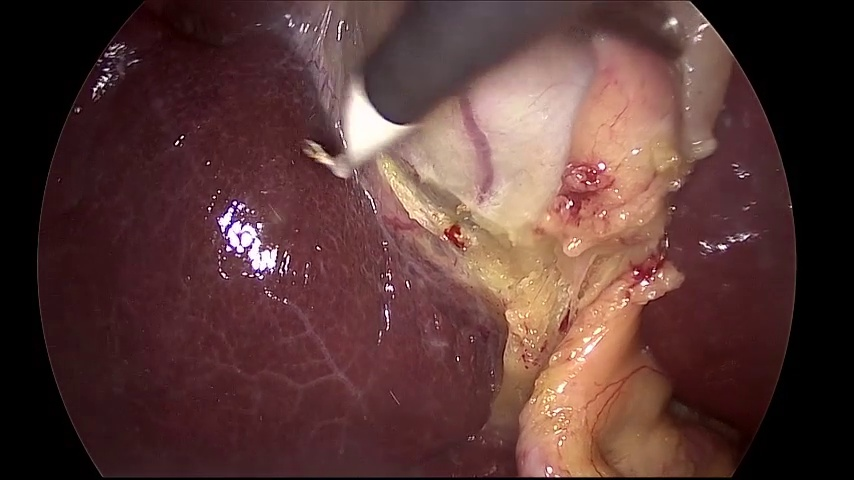
\includegraphics[scale=0.3]{video01-first-tool-frame-003375.jpg}
\caption{Frame 3375 de \texttt{video01}, aos 135,00 s. O detector previu \texttt{hook} com confiança 0,926, confirmado em três frames consecutivos. A imagem original não exibe a caixa predita; ver metadados no Anexo~\ref{sec:metadados-deteccao}.}
\label{fig:primeira-deteccao}
\end{figure}

\subsection{Relatório Markdown da primeira detecção}\label{sec:relatorio-deteccao}

\lstinputlisting[style=terminal,inputencoding=utf8/latin1]{video01-first-tool-frame-003375.md}

\subsection{Metadados JSON da primeira detecção}\label{sec:metadados-deteccao}

\lstinputlisting[style=terminal,inputencoding=utf8/latin1]{video01-first-tool-frame-003375.json}

\subsection{Saída do terminal da execução do pipeline de áudio}\label{sec:execucao-audio}

\lstinputlisting[style=terminal,inputencoding=utf8/latin1]{audio-execucao-terminal.txt}

\end{document}
